\documentclass[utf8,xcolor=table]{beamer}

\usepackage[T2A]{fontenc}
\usepackage[utf8]{inputenc}
\usepackage[english,russian]{babel}
\usepackage{minted}
\usepackage{ulem}
\usepackage{cmap}
\usepackage{multirow}

\hypersetup{colorlinks,linkcolor=blue,urlcolor=blue}

\mode<presentation>{
	\usetheme{CambridgeUS}
}

\renewcommand{\t}[1]{\ifmmode{\mathtt{#1}}\else{\texttt{#1}}\fi}

\title{Многопоточность}
\author{Егор Суворов}
\institute[СПб АУ]{Курс <<Парадигмы и языки программирования>>, подгруппа 3}
\date[19.10.2016]{Среда, 19 октября 2016 года}

\setlength{\arrayrulewidth}{1pt}

\begin{document}

\begin{frame}
\titlepage
\end{frame}

\begin{frame}{План занятия}
	\tableofcontents
\end{frame}

\section{Параллельные вычисления}
\subsection{Зачем}

\begin{frame}
	\tableofcontents[currentsection,currentsubsection]
\end{frame}

\begin{frame}{Скорость вычислений}
	\begin{itemize}
		\item Хочется обрабатывать всё б\'{о}льшие объёмы информации всё быстрее.
		\item Пример: эмуляция движений воздуха на планете Земля за ближайшие 48 часов (прогноз погоды).
		\item Пока работает эмпирический \href{https://ru.wikipedia.org/wiki/\%D0\%97\%D0\%B0\%D0\%BA\%D0\%BE\%D0\%BD\_\%D0\%9C\%D1\%83\%D1\%80\%D0\%B0}{закон Мура}: каждые два года плотность транзисторов удваивается.
		\item Раньше это означало увеличение частоты процессора в два раза.
		\item Уже нет: процессор с частотой 2.8 ГГц был представлен в 2004 году (Pentium 4 Prescott).
		\item С тех пор скорость работы повышалась, но другими способами: размер кэша, скорость памяти, периферии...
		\item Уже уткнулись в ограничения размера процессора из-за скорости света.
	\end{itemize}
\end{frame}

\begin{frame}[fragile]{Параллелизм}
	\begin{itemize}
		\item Иногда можно работать быстрее, не увеличивая частоту, распараллелив команды:
\begin{minted}{cpp}
int x = a * b * 10;  // Нужен блок умножения.
int y = a / b;       // Нужен блок деления.
\end{minted}
		\item Процессоры умеют это автоматически детектировать без участия программистов.
		\item Компиляторы умеют передвигать операции так, чтобы процессору было проще.
		\item В последние годы активно появляются многоядерные процессоры: впихнуть второе ядро оказалось проще оптимизации физических процессов.
		\item Также можно использовать мощь б\'{о}льшего числа компьютеров (\href{https://ru.wikipedia.org/wiki/Folding@home}{Folding@Home}).
	\end{itemize}
\end{frame}

\begin{frame}{На домашнем компьютере}
	Идеи распараллеливания полезны и где-то, кроме ускорения:
	\begin{itemize}
		\item
			Обычные задачи дома не требуют большой вычислительной мощи:
			\begin{itemize}
				\item Процесс обычно ждёт реакции пользователя, диска или сети.
				\item Вычисления длятся не больше нескольких секунд.
			\end{itemize}
		\item Хочется свободно переключаться между приложениями и слушать музыку в фоне.
		\item Если есть ресурсоёмкая задача, нестрашно, если она будет выполняться чуть медленнее.
		\item На телефоне одно ядро может целиком отрисовывать нетормозящий интерфейс, а другое "--- производить вычисления.
	\end{itemize}
\end{frame}

\subsection{Как}
\begin{frame}[fragile]{Параллельные алгоритмы}
	\begin{itemize}
		\item Некоторые алгоритмы параллелятся просто:
\begin{minted}{cpp}
int sum = 0;
for (int x : values) sum += x;
\end{minted}
		\item Некоторые "--- естественно и на уровне железа:
\begin{minted}{cpp}
char buf1[100], buf2[100];
fread(file_on_disk1, 1, sizeof buf1, buf1);
fread(file_on_disk2, 1, sizeof buf2, buf2);
\end{minted}
		\item Некоторые не параллелятся:
\begin{minted}{cpp}
int steps = 0;
for (int x = 0; x != 0; x = f(x)); steps++;
\end{minted}
		\item Надо писать специальные алгоритмы для распределённых вычислений.
	\end{itemize}
\end{frame}

\begin{frame}{Иллюстрация}
	\begin{center}
		
\includegraphics[height=6cm]{cpus-joke.jpg}

		Простое добавление ядер не увеличивает производительность!
	\end{center}
\end{frame}

\begin{frame}{В прикладном хозяйстве}
	\begin{itemize}
		\item Современные ОС различают \textit{потоки} и \textit{процессы}.
		\item Процесс "--- это обычно одно приложение (браузер, IDE, веб-сервер...), у которого может быть много потоков.
		\item Например: у браузера один поток на вкладку; у веб-сервера "--- один поток на клиента.
		\item Изначально у процесса есть только один поток (\textit{главный}), он может создавать другие.
		\item Более строго: процесс "--- это некоторое множество потоков, у которых общая память и другие ресурсы (открытые файлы).
		\item Поток "--- это что-то, выполняющее некий код (есть отдельный стек, свои данные в регистрах процессора, свой код).\
	\end{itemize}
\end{frame}

\begin{frame}{С точки зрения программиста}
	\begin{itemize}
		\item На разных ОС разные методы для работы с процессами или потоками.
		\item Напрямую API уровня ОС, как обычно, никто не использует.
		\item В языке высокого уровня (Java, Python) обычно есть соответствующая библиотека.
		\item Также есть другие классические библиотеки и стандарты:
			\begin{itemize}
				\item pthread "--- Posix Thread, стандарт в C. Будем использовать.
				\item OpenMP "--- высокоуровневое распараллеливание для C/C++/Fortran.
				\item CUDA "--- вычисления на графических картах (ядер тысячи, но они умеют меньше, чем CPU).
			\end{itemize}
	\end{itemize}
\end{frame}

\begin{frame}[fragile]{Типичный псевдокод-1}
\begin{minted}{cpp}
void draw() {
    while (true) {
        wait_for_events();
        process_updates();
        process_mouse_events();
        repaint();
    }
}
int main() {
    Thread draw_thread(draw);
    draw_thread.start();
    // ...
    add_rectangle(10, 10, 30, 40);
    // ...
}
\end{minted}
\end{frame}

\begin{frame}[fragile]{Типичный псевдокод-2}
\begin{minted}{cpp}
void process_client(Client client) {
    string request = client.read();
    string answer = "I've got " + request;
    client.write(answer);
}
int main() {
    while (true) {
        Client client = get_next_client();
        Thread(process+client, client).start();
    }
}
\end{minted}
\end{frame}

\begin{frame}[fragile]{Типичный псевдокод-3}
\begin{minted}{cpp}
void merge_sort(int l, int r) {
    if (l + 1 == r) return;
    Thread t1(merge_sort, l, (l + r) / 2);
    Thread t2(merge_sort, (l + r) / 2, r);
    t1.start(); t2.start(); // Запускаем потоки.
    t1.join(); t2.join();   // Ждём завершения.
    merge(l, r);
}
\end{minted}
\end{frame}

\section{Практические грабли}
\subsection{Простое приложение на pthread}

\begin{frame}
	\tableofcontents[currentsection,currentsubsection]
\end{frame}

\begin{frame}{Что такое pthread}
	\begin{itemize}
		\item Стандартный интерфейса функций для работы с потоками (POSIX Threads).
		\item Есть реализации под Windows, Linux и другие ОС.
		\item Стандарт при разработке программ на C.
		\item Имена функций и типов начинаются с \t{pthread\_}.
		\item В Linux можно получить справку, набрав \t{man <имя функции>} в консоли.
		\item Под остальными "--- то же самое, но в гугле.
	\end{itemize}
\end{frame}

\begin{frame}[fragile]{Пример кода}
\begin{minted}{cpp}
void* worker(void* arg) {
    printf("Hello from thread! arg=%d\n", *(int*)arg);
    *(int*)arg += 10;
    return arg;
}
int main(void) {
    pthread_t id;
    int data = 1234;
    assert(pthread_create(&id, NULL, worker, &data) == 0);
    void* retval;
    assert(pthread_join(id, &retval) == 0);
    assert(retval == &data);
    printf("data is %d\n", data);
    return 0;
}
\end{minted}
\end{frame}

\begin{frame}{Как живут потоки}
	\begin{itemize}
		\item При создании потока при помощи \t{pthread\_create} указывается функция и её аргумент "--- один указатель на что угодно.
		\item Вернуть функция тоже может указатель на что угодно.
		\item Поток завершается, когда функция делает \t{return} или \t{pthread\_exit}.
		\item Указатель на поток хранится в переменной типа \t{pthread\_t}.
		\item При создании потока он сразу начинает выполняться.
		\item \t{pthread\_join} делает следующее:
			\begin{enumerate}
				\item Ждёт окончания работы потока.
				\item Освобождает все ресурсы потока (стек).
				\item Возвращает то, что вернула функция потока.
			\end{enumerate}
		\item Когда \t{main} делает \t{return 0} или вы вызываете \t{exit(0)}, умирает весь процесс со всеми потоками.
		\item Но в \t{main} можно сделать \t{pthread\_exit}, если очень хочется, тогда процесс не умрёт, пока живы потоки.
	\end{itemize}
\end{frame}

\begin{frame}[fragile]{Упражнение: сборка кода}
	\begin{enumerate}
		\item Качаем решение с \href{https://github.com/yeputons/fall-2016-paradigms/raw/master/161019/sources/01-simple.c}{GitHub}.
		\item \texttt{gcc 01-simple.c -o 01-simple -Wall -Wextra -Werror} или аналог в вашей IDE.
		\item \texttt{./01-simple}
		\item Ожидаемый вывод:
\begin{verbatim}
Hello from thread! arg=1234
data is 1244
\end{verbatim}
	\end{enumerate}
\end{frame}

\begin{frame}{Несколько замечаний про C}
	\begin{itemize}
		\item На языке C лучше включить все предупреждения компилятора (warnings), в GCC это делают ключи \t{-Wall}, \t{-Wextra}.
		\item Если вы включили предупреждения "--- их лучше сразу трактовать как ошибки (\t{-Werror}), иначе быстро научитесь их игнорировать.
		\item Если аргумент функции не используется, после него в GCC надо писать \t{\_\_attribute\_\_((unused))}.
		\item Из функции всегда надо что-то вернуть (хотя бы \t{NULL}).
		\item \href{http://codeforces.com/blog/entry/17747}{Никогда} не начинайте название переменной с нижнего подчёркивания!
		\item Константы задаются при помощи \t{\#define SOME\_CONST (value)}.
	\end{itemize}
\end{frame}

\begin{frame}[t]{Иллюстрация}
	\begin{center}
		
\includegraphics[scale=0.5]{no-werror-meme.jpg}
	\end{center}
\end{frame}

\begin{frame}[t]{Несколько замечаний про pthread}
	Про потоки и pthread:
	\begin{itemize}
		\item Использовать \t{void* arg} и возвращаемое значение для передачи данных необязательно.
		\item Вся память внутри процесса одинаково доступна всем потокам на чтение и запись.
		\item \t{void* arg} возникает только тогда, когда надо запустить потоки на разных данных.
		\item Что произойдёт, если мы забудем \t{join} и \t{main} завершится до начала \t{worker}?
			\only<2->{Неопределённое поведение "--- \t{worker} попытается изменить переменную \t{data}, которая уже исчезла.}
	\end{itemize}
\end{frame}

\begin{frame}{Кто освобождает ресурсы?}
	На самом деле в pthread есть два типа потоков: joinable и detached.

	Joinable:
	\begin{itemize}
		\item Тип по умолчанию.
		\item На таком потоке должен быть ровно один раз вызыван метод \t{pthread\_join}, который освободит ресурсы и сообщит, что поток вернул.
		\item Если не вызвать "--- ресурсы не будут освобождены до конца программы.
		\item Если вызвать дважды "--- второй вызов может уронить программу или вернуть неверный результат.
	\end{itemize}

	Detached:
	\begin{itemize}
		\item Система автоматически освободит ресурсы как только поток завершится.
		\item Нельзя вызывать \t{pthread\_join} и получать возвращаемое значение "--- его негде хранить после окончания работы.
	\end{itemize}
\end{frame}

\begin{frame}{В других системах}
	\begin{itemize}
		\item Joinable/detached также используется в Java.
		\item В Windows (не в pthread под Windows!) другая концепция:
			\begin{itemize}
				\item Указатель на поток "--- сложный объект, который надо запрашивать у ОС и освобождать (как \t{FILE*}), а не просто переменная.
				\item Ресурсы потока освобождаются, когда он завершился и на него больше нет указателей.
				\item Нет разделения joinable/detached.
				\item Если кто-то может спросить состояние потока "--- у него есть указатель, значит, ресурсы потока ещё не освобождены.
			\end{itemize}
	\end{itemize}
\end{frame}

\begin{frame}{Упражнение}
	\begin{enumerate}
		\item Измените код так, чтобы \t{data} стала глобальной переменной (после этого \t{arg} не нужен).
		\item Вызовите \t{pthread\_detach} на втором потоке после запуска.
		\item Убедитесь, что программа упала.
		\item Уберите вызов \t{pthread\_join} и \t{printf} из основного потока.
		\item Убедитесь, что второй поток не всегда успевает отработать.
		\item Добавьте вызов \t{pthread\_exit} в \t{main}.
		\item Убедитесь, что после приложение перестало закрываться до окончания работы всех потоков.
	\end{enumerate}
	\href{https://github.com/yeputons/fall-2016-paradigms/raw/master/161019/sources/02-detached.c}{Код}
\end{frame}

\subsection{Состояние гонки}

\begin{frame}
	\tableofcontents[currentsection,currentsubsection]
\end{frame}

\begin{frame}{Упражнение}
	\begin{itemize}
		\item Возьмите \href{https://github.com/yeputons/fall-2016-paradigms/raw/master/161019/sources/03-writeln-single.c}{код}.
		\item При желании можете скачать \href{https://github.com/yeputons/fall-2016-paradigms/raw/master/161019/sources/Makefile}{Makefile}.
		\item Убедитесь, что на экран выводится строка.
		\item Запустите второй поток, который выводит на экран другую строку.
		\item Найдите место, где первая строка сменяется второй.
		\item Удивитесь.
	\end{itemize}
	\href{https://github.com/yeputons/fall-2016-paradigms/raw/master/161019/sources/04-writeln-race.c}{Код}
\end{frame}

\begin{frame}{Объяснение}
	\begin{itemize}
		\item
			Потоки выполняют команды <<одновременно>>.
			Если есть доступ к общему ресурсу (экран), то порядок не определить.
		\item
			Поэтому символы выводятся вперемешку.
		\item
			\textit{Состояние гонки} (\textit{race condition}) "--- это когда результат работы зависит от того, в каком порядке потоки выполняли команды.
		\item
			Самая популярная ошибка у начинающих.
		\item
			Операция называется \textit{атомарной}, если она всегда выполняется <<за один такт>>,
			то есть другие потоки не видят её частично выполненной.
		\item
			\t{writeln} выше не атомарна.
	\end{itemize}
\end{frame}

\begin{frame}{Упражнение}
	\begin{enumerate}
		\item Сделайте счётчик:
			\begin{itemize}
				\item Второй поток в цикле увеличивает глобальную переменную \t{data} до $N = 5 \cdot 10^8$.
				\item Основной поток (\t{main}) выводит на экран текущее значение \t{data} в цикле $M = 1000$ раз.
				\item Отключите оптимизации компилятора (ключ \t{-O2} или схожий не нужен).
			\end{itemize}
		\item Убедитесь, что программа выводит на экране увеличивающиеся значения, а в конце "--- $N$.
		\item Поиграйте со значением $M$, чтобы убедиться, что в конце всегда выводится $N$.
		\item Сделайте так, чтобы основной поток выводил на экран только чётные значения \t{data} и увеличьте $M$.
		\item Что теперь происходит?
	\end{enumerate}
	Мой код:
	\href{https://github.com/yeputons/fall-2016-paradigms/raw/master/161019/sources/05-counter.c}{счётчик},
	\href{https://github.com/yeputons/fall-2016-paradigms/raw/master/161019/sources/06-even-counter.c}{чётный счётчик}.
\end{frame}

\begin{frame}{Объяснение}
	Возможная последовательность действий:
	\begin{itemize}
		\item Основной поток: \t{if (data \% 2 == 0)} $\to \t{true}$.
		\item Второй поток: \t{data++}.
		\item Основной поток: \t{printf}.
	\end{itemize}
	Как исправить?
	\pause
	\begin{itemize}
		\item Можно на каждой итерации записать значение \t{data} в локальную \t{data\_snapshot} (снимок) и работать с ним.
		\item Работает только если чтение одной переменной атомарно.
		\item Не работает, если у нас много переменных мы не можем сделать атомарный снимок (классическая задача).
	\end{itemize}
\end{frame}

\begin{frame}{Иллюстрация}
	\begin{center}
		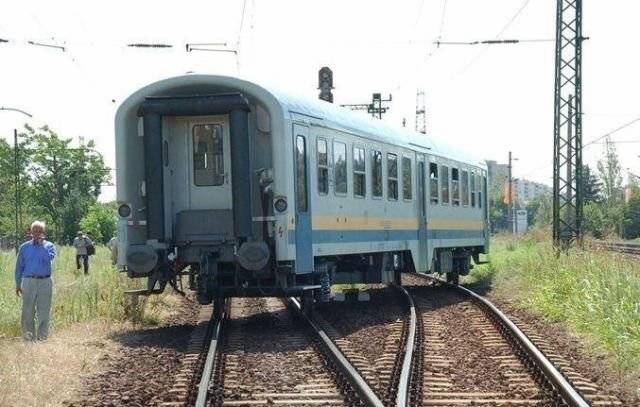
\includegraphics[scale=0.6]{race-condition.jpg}
	\end{center}
\end{frame}

\subsection{Гонка данных}
\begin{frame}{Упражнение}
	\begin{itemize}
		\item Добавьте снятие снимков в свой счётчик.
		\item Убедитесь, что все значения теперь чётные.
		\item Запустите второй поток-счётчик, который тоже увеличивает \t{data}.
		\item Что произошло?
	\end{itemize}
	Мой код:
	\href{https://github.com/yeputons/fall-2016-paradigms/raw/master/161019/sources/07-even-counter-snapshot.c}{счётчик со снимками},
	\href{https://github.com/yeputons/fall-2016-paradigms/raw/master/161019/sources/08-two-threads.c}{два счётчика}.
\end{frame}

\begin{frame}{Объяснение}
	\begin{enumerate}
		\item На уровне железа \t{data++} происходит так:
			\begin{itemize}
				\item Считай значение \t{data} из памяти.
				\item Прибавь единицу.
				\item Положи \t{data+1} на то же место в памяти.
			\end{itemize}
		\item
			Порядок операций между разными потоками произвольный.
			\begin{center}
				\begin{tabular}{cc}
					\begin{tabular}{l|c}
						Операция & \t{data} \\ \hline
						1: \t{read} $\to 10$ & 10 \\
						1: \t{+1} $\to 11$ & 10 \\
						1: \t{write(11)} & 11 \\
						2: \t{read} $\to 11$ & 11 \\
						2: \t{+1} $\to 12$ & 11 \\
						2: \t{write(12)} & 12 \\
					\end{tabular}
					&
					\begin{tabular}{l|c}
						Операция & \t{data} \\ \hline
						1: \t{read} $\to 10$ & 10 \\
						1: \t{+1} $\to 11$ & 10 \\
						2: \t{read} $\to 10$ & 10 \\
						2: \t{+1} $\to 11$ & 10 \\
						1: \t{write(11)} & 11 \\
						2: \t{write(11)} & 11 \\
					\end{tabular}
				\end{tabular}
			\end{center}
	\end{enumerate}
\end{frame}

\begin{frame}{А что вообще атомарно?}
	\begin{center}
		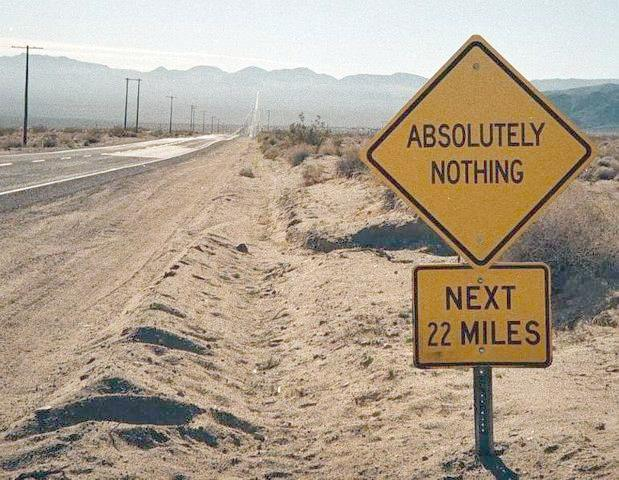
\includegraphics[scale=0.4]{absolutely-nothing.jpg}
	\end{center}
\end{frame}

\begin{frame}{Полезные советы}
	\begin{itemize}
		\item
			Что атомарно "--- очень сильно зависит от платформы, языка и ключей компиляции
			(<<модель памяти>>).
		\item Не пытайтесь угадать.
		\item Не пытайтесь самостоятельно писать код, зависящий от атомарности.
		\item В некоторых языках бывает \t{AtomicInteger} и похожие структуры.
		\item За ними тоже надо аккуратно следить, обычно не используют.
	\end{itemize}
\end{frame}


\end{document}
